% Vietnamese translation for OI Public Library
% Source-PDF: IOI中国国家候选队论文/2000/方奇论文.pdf
\documentclass[11pt]{article}
\usepackage{oipl-vn}
\usepackage{tikz}

\title{Quy hoạch động}
\author{Fang Qi}
\date{}

\begin{document}
\maketitle

\origtitle{Dynamic programming}
\sourcepath{IOI China candidate team papers / 2000 / Fang Qi.pdf}

\paragraph{Từ khóa.}
Giai đoạn; trạng thái; quyết định; công thức truy hồi.

\section*{Tóm tắt}

Quy hoạch động là một phương pháp tư duy để giải các bài toán tối ưu hóa
quyết định nhiều giai đoạn. Chữ ``động'' ở đây nghĩa là: trong quá trình ra
quyết định qua nhiều giai đoạn, theo một thứ tự nào đó, mỗi quyết định được
chọn ở từng bước sẽ lập tức gây ra một phép chuyển trạng thái, và cuối cùng
tạo ra một dãy quyết định trong các trạng thái biến đổi. Quy hoạch động nhằm
làm cho dãy quyết định ấy đạt tối ưu dưới một số điều kiện nhất định. Gần đây,
tư tưởng quy hoạch động xuất hiện thường xuyên trong nhiều loại kỳ thi tin
học, và ứng dụng của nó ngày càng được coi trọng. Bài viết này thảo luận cách
vận dụng tư tưởng quy hoạch động để thiết kế những mô hình toán học hữu hiệu
cho việc giải bài.

\section{Mô tả toán học của bài toán quy hoạch động}

Trước hết ta xét một bài toán quyết định nhiều giai đoạn đơn giản.

\subsubsection*{Ví dụ 1}

Hiện có một bản đồ; mỗi nút biểu diễn một thành phố, mỗi cạnh nối hai nút biểu
diễn một con đường, và số ghi trên cạnh là khoảng cách giữa hai thành phố. Như
trong Hình 1, hãy tìm đường đi ngắn nhất từ nút $1$ đến nút $10$.

\paragraph{Hình 1.}
Hình dưới là đồ thị phân lớp gồm năm giai đoạn
\[
  \{1\},\quad \{2,3\},\quad \{4,5,6\},\quad \{7,8,9\},\quad \{10\}.
\]
Các cạnh chỉ nối giữa hai giai đoạn kề nhau, và số trên cạnh là chi phí đi
giữa hai thành phố.

\begin{center}
\begin{tikzpicture}[
  v/.style={circle,draw,minimum size=0.58cm,inner sep=0pt,font=\small},
  edge/.style={->,black!80,thick},
  stage/.style={black!70,thick},
  every node/.style={font=\scriptsize},
  x=0.9cm,y=0.9cm
]
  \node[v] (n1) at (0,0) {1};
  \node[v] (n2) at (1.6,1.0) {2};
  \node[v] (n3) at (1.6,-1.0) {3};
  \node[v] (n4) at (3.2,1.55) {4};
  \node[v] (n5) at (3.2,0) {5};
  \node[v] (n6) at (3.2,-1.55) {6};
  \node[v] (n7) at (4.9,1.55) {7};
  \node[v] (n8) at (4.9,0) {8};
  \node[v] (n9) at (4.9,-1.55) {9};
  \node[v] (n10) at (6.6,0) {10};

  \foreach \x/\label in {0/GĐ 1,1.6/GĐ 2,3.2/GĐ 3,4.9/GĐ 4,6.6/GĐ 5}
    \node[font=\scriptsize] at (\x,2.35) {\label};
  \foreach \x in {0.8,2.4,4.05,5.75} \draw[stage] (\x,-2.05)--(\x,2.05);

  \draw[edge] (n1)--node[above]{4}(n2);
  \draw[edge] (n1)--node[below]{2}(n3);
  \draw[edge] (n2)--node[above]{1}(n4);
  \draw[edge] (n2)--node[below left]{5}(n5);
  \draw[edge] (n3)--node[above left]{3}(n4);
  \draw[edge] (n3)--node[above]{4}(n5);
  \draw[edge] (n3)--node[below]{3}(n6);
  \draw[edge] (n4)--node[right]{6}(n9);
  \draw[edge] (n5)--node[above]{7}(n7);
  \draw[edge] (n5)--node[above]{5}(n8);
  \draw[edge] (n6)--node[below right]{5}(n8);
  \draw[edge] (n7)--node[above right]{3}(n10);
  \draw[edge] (n8)--node[above]{4}(n10);
  \draw[edge] (n9)--node[below right]{6}(n10);
\end{tikzpicture}
\end{center}

Bài toán này có thể giải bằng cách vét cạn thông thường: liệt kê mọi đường đi
từ nút $1$ đến nút $10$, tính độ dài, rồi so sánh để tìm đường nhỏ nhất. Tuy
có thể giải được, nhưng khi số nút tăng lên, lượng tính toán của cách này tăng
theo cấp số mũ, nên hiệu quả rất thấp.

Phân tích Hình 1, ta thấy các đặc điểm sắp xếp của các nút:
\begin{enumerate}
  \item Có thể chia các nút thành $5$ giai đoạn.
  \item Mỗi nút ở một giai đoạn chỉ nối với các nút ở giai đoạn kề bên, không
  có cạnh vượt giai đoạn hoặc cạnh trong cùng một giai đoạn; chẳng hạn không
  có cạnh nối nút $1$ với nút $4$, hay nút $4$ với nút $5$.
  \item Ngoài điểm đầu $1$ và điểm cuối $10$, các nút ở những giai đoạn khác
  vừa là điểm cuối của giai đoạn trước, vừa là điểm đầu của giai đoạn sau.
  Chẳng hạn các nút $4,5,6$ ở giai đoạn thứ ba vừa là điểm cuối của một nút
  nào đó trong các nút $2,3$ ở giai đoạn trước, vừa là điểm đầu của một nút
  nào đó trong các nút $7,8,9$ ở giai đoạn sau.
\end{enumerate}

Theo các đặc điểm trên, xét nút $5$ ở giai đoạn thứ ba. Trong hai đường
$1-2-5$ và $1-3-5$, đường sau có chi phí nhỏ hơn đường trước. Giả sử đường
ngắn nhất cần tìm từ nút $1$ đến nút $10$ phải đi qua nút $5$; khi đó giữa
nút $1$ và nút $5$ ta sẽ chọn đường nào? Rõ ràng, bất kể từ nút $5$ về sau đi
như thế nào, việc chọn $1-3-5$ ở phần trước luôn tốt hơn $1-2-5$. Nói cách
khác, khi đã xác định nút ở một giai đoạn, sự phát triển của các tuyến đường
ở những giai đoạn sau không chịu ảnh hưởng bởi các giai đoạn trước nút ấy.
Ngược lại, quyết định tối ưu để đi đến nút ấy cũng không chịu ảnh hưởng của
phần phát triển sau nút ấy.

Vì vậy ta có thể tách bài toán gốc thành nhiều bài toán nhỏ: bắt đầu từ giai
đoạn $1$, lần lượt tính khoảng cách ngắn nhất từ nút $1$ đến các nút ở giai
đoạn $2,3,4,5$, cuối cùng nhận được đáp án. Trong quá trình tính, quyết định
để đi đến một nút ở một giai đoạn chỉ phụ thuộc vào kết quả tính của giai
đoạn trước, không phụ thuộc vào yếu tố khác. Chẳng hạn, nếu đã biết giá trị
tối ưu từ nút $1$ đến nút $5$ là $6$, đến nút $6$ là $5$, thì để tính giá trị
tối ưu đến nút $8$ ở giai đoạn sau, chỉ cần so sánh
\[
  \min\{6+5,\;5+5\}.
\]
Như vậy, vận dụng tư tưởng quy hoạch động giúp tiết kiệm rất nhiều tính toán.
Có thể thấy quy hoạch động là một phương pháp hiệu quả để giải loại bài toán
quyết định nhiều giai đoạn này.

\section{Các khái niệm và thuật ngữ chính trong quy hoạch động}

\begin{enumerate}
  \item \term{Giai đoạn}: chia bài toán thành vài khâu có thứ tự và liên hệ
  với nhau; các khâu ấy được gọi là giai đoạn.
  \item \term{Trạng thái}: vị trí xuất phát của một giai đoạn được gọi là
  trạng thái. Thông thường một giai đoạn chứa nhiều trạng thái. Trong Hình 1,
  giai đoạn $3$ có ba trạng thái là các nút $4,5,6$.
  \item \term{Quyết định}: lựa chọn làm cho một trạng thái ở một giai đoạn
  chuyển thành một trạng thái nào đó ở giai đoạn tiếp theo.
  \item \term{Chiến lược}: trong toàn bộ quá trình từ điểm đầu đến điểm cuối,
  dãy quyết định tạo bởi các quyết định ở từng đoạn được gọi là chiến lược
  toàn quá trình, gọi tắt là chiến lược.
  \item \term{Phương trình chuyển trạng thái}: điểm cuối của giai đoạn trước
  là điểm đầu của giai đoạn sau, và quyết định ở giai đoạn trước dẫn ra trạng
  thái của giai đoạn sau. Quan hệ này mô tả quy luật biến đổi trạng thái từ
  giai đoạn $k$ sang giai đoạn $k+1$, nên được gọi là phương trình chuyển
  trạng thái.
  \item \term{Hàm mục tiêu và khái niệm tối ưu hóa}: hàm mục tiêu là tiêu
  chuẩn đo mức tốt xấu của quá trình quyết định nhiều giai đoạn. Khái niệm tối
  ưu hóa là tìm một con đường dưới những điều kiện nhất định, sao cho sau các
  phép toán được xác định bởi tính chất cụ thể của đề bài, tổng hiệu quả của
  toàn quá trình đạt tối ưu.
\end{enumerate}

\section{Điều kiện cần thỏa để dùng quy hoạch động}

Bất kỳ phương pháp tư duy nào cũng có giới hạn nhất định; vượt khỏi điều kiện
đặc thù thì nó mất tác dụng. Tương tự, quy hoạch động không phải là vạn năng.
Vậy dùng quy hoạch động cần thỏa những điều kiện nào? Cần thỏa nguyên lý tối
ưu và tính không hậu hiệu.

\subsection{Nguyên lý tối ưu}

Nguyên lý tối ưu có thể phát biểu như sau: một chiến lược tối ưu có tính chất
rằng, bất kể trạng thái và quyết định trong quá khứ ra sao, đối với trạng thái
đã được hình thành bởi các quyết định phía trước, những quyết định còn lại
phải tạo thành một chiến lược tối ưu. Nói ngắn gọn, chiến lược con của một
chiến lược tối ưu luôn là tối ưu.

\paragraph{Hình 2.}
Hình dưới minh họa một đường từ $A$ đến $C$ được tách thành đoạn $I$ từ $A$
đến $B$ và đoạn $J$ từ $B$ đến $C$, đồng thời vẽ một đường thay thế $J'$ từ
$B$ đến $C$.

\begin{center}
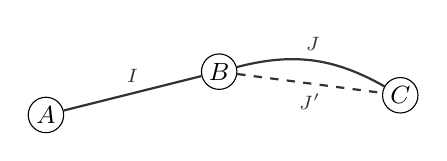
\begin{tikzpicture}[
  v/.style={circle,draw,minimum size=0.45cm,inner sep=0pt,font=\small},
  edge/.style={black!80,thick},
  every node/.style={font=\scriptsize}
]
  \node[v] (a) at (0,0) {$A$};
  \node[v] (b) at (2.2,0.55) {$B$};
  \node[v] (c) at (4.5,0.25) {$C$};
  \draw[edge] (a)--node[above]{\(I\)}(b);
  \draw[edge] (b) to[bend left=22] node[above]{\(J\)} (c);
  \draw[edge,dashed] (b)--node[below]{\(J'\)}(c);
\end{tikzpicture}\\[-0.2em]
{\small Hình 2. Minh họa nguyên lý tối ưu.}
\end{center}

Trong Hình 2, nếu đường gồm $I$ và $J$ là đường tối ưu từ $A$ đến $C$, thì theo
nguyên lý tối ưu, $J$ nhất định là đường tối ưu từ $B$ đến $C$. Điều này có
thể chứng minh bằng phản chứng: giả sử có một đường khác $J'$ là đường tối ưu
từ $B$ đến $C$, thì đường từ $A$ đến $C$ dùng $I$ và $J'$ sẽ tốt hơn đường dùng
$I$ và $J$, mâu thuẫn với giả thiết của bài toán gốc. Do đó $J$ phải là đường
tối ưu từ $B$ đến $C$.

Nguyên lý tối ưu là nền tảng của quy hoạch động. Với bất kỳ bài toán nào, nếu
không có sự hỗ trợ của nguyên lý tối ưu thì không thể tính bằng phương pháp
quy hoạch động.

\subsection{Tính không hậu hiệu}

``Các bước trong quá khứ chỉ có thể ảnh hưởng đến sự phát triển tương lai
thông qua trạng thái hiện tại; trạng thái hiện tại là bản tổng kết của lịch
sử.'' Đặc điểm này cho thấy quy hoạch động chỉ thích hợp để giải những bài
toán mà quyết định hiện tại không phụ thuộc vào trạng thái quá khứ. Một trạng
thái, dù xuất hiện ở vị trí nào trong chiến lược, đều có địa vị như nhau và
có thể áp dụng cùng một chiến lược; đó chính là nội hàm của tính không hậu
hiệu.

Từ trên có thể thấy, nguyên lý tối ưu và tính không hậu hiệu là hai điều kiện
mà quy hoạch động phải thỏa.

\section{Phương pháp tính của quy hoạch động}

Với một bài toán, cụ thể phải vận dụng quy hoạch động như thế nào?
\begin{enumerate}
  \item Trước hết, phân tích đề bài, xem bài toán có thỏa nguyên lý tối ưu và
  tính không hậu hiệu hay không.
  \item Tiếp theo, xác định các giai đoạn, trạng thái và điều kiện ràng buộc
  trong đề.
  \item Suy ra phương trình cơ bản giữa các trạng thái ở các giai đoạn rồi
  tiến hành tính toán.
\end{enumerate}

Cách giải cụ thể có nhiều loại.

\subsection{Quy hoạch động tiến và lùi}

Tiến và lùi ở đây nghĩa là xuất phát từ điểm đầu, truy hồi từng lớp cho đến
điểm cuối, hoặc xuất phát từ điểm cuối và giải ngược lại. Về bản chất, hai
phương pháp này giống nhau; khi giải bài cụ thể, ta có thể chọn theo tình
huống thực tế.

\subsubsection*{Ví dụ 2: xếp hàng mua vé}

\paragraph{Mô tả bài toán.}
Một buổi hòa nhạc sắp diễn ra. Hiện có $N$ người hâm mộ xếp hàng mua vé, với
$0<N\le 200$; mỗi người mua một vé. Quầy vé quy định mỗi người mỗi lần nhiều
nhất chỉ được mua hai vé. Giả sử người hâm mộ thứ $i$ mua một vé cần thời
gian $T_i$ ($1\le i\le n$). Hai người hâm mộ kề nhau trong hàng, tức người
thứ $j$ và người thứ $j+1$, cũng có thể để một trong hai người mua hai vé, còn
người kia khỏi phải xếp hàng; khi đó thời gian mua hai vé của hai người này
trở thành $R_j$. Nếu $R_j<T_j+T_{j+1}$ thì cách này có thể rút ngắn thời gian
chờ của những người phía sau và tăng tốc toàn bộ quá trình bán vé. Cho $N$,
các $T_j$ và $R_j$, hãy tìm thời gian ngắn nhất và phương án để mọi người đều
mua được vé.

\paragraph{Giải bài toán.}
Các giai đoạn của bài này rất rõ ràng: chỉ cần chia theo thứ tự trong hàng.
Cách mua vé chỉ có hai loại, hoặc mỗi người mua một vé, hoặc một người mua hai
vé; toàn bộ quá trình sắp theo một đường thẳng. Để thời gian mua vé của $i$
người đầu là ngắn nhất, chỉ cần xét cách mua vé của $i$ người đầu, không liên
quan đến những người phía sau trong hàng. Hơn nữa, hiển nhiên trong chiến
lược tối ưu, bất kỳ $m$ quyết định liên tiếp nào cũng phải là tối ưu. Do đó
bài toán thỏa nguyên lý tối ưu và tính không hậu hiệu, nên có thể dùng quy
hoạch động.

Vậy xây dựng công thức truy hồi thế nào? Lấy thời gian ngắn nhất cần thiết
đến hết mỗi người làm giá trị trạng thái, ký hiệu là $f(i)$. Khi đó
\[
  f(i)=\min\{f(i-1)+T_i,\;f(i-2)+R_{i-1}\},
\]
với điều kiện đầu
\[
  f(0)=0,\qquad f(1)=T_1.
\]
Như vậy đi từ trước ra sau chỉ cần duyệt một lần.

Phân tích trên đi từ trước ra sau. Thực ra suy ngược cũng tương tự. Gọi
$f(i)$ là thời gian tối thiểu còn cần để bán hết vé khi việc bán đã tới người
thứ $i$. Khi đó công thức truy hồi là
\[
  f(i)=\min\{f(i+1)+T_i,\;f(i+2)+R_i\},
\]
tính ngược từ sau ra trước với điều kiện đầu
\[
  f(n)=T_n,\qquad f(n+1)=0.
\]

Dùng quy hoạch động tiến hay lùi phụ thuộc vào tình huống thực tế; cách nào
trực quan và đơn giản hơn thì dùng cách ấy.

\subsection{Bài toán có giai đoạn ẩn}

Chia giai đoạn là một khâu quan trọng trong quy hoạch động. Nhưng có những
bài toán không có giai đoạn rõ ràng mà vẫn thỏa nguyên lý tối ưu; khi đó giải
ra sao? Ta xét một ví dụ.

\subsubsection*{Ví dụ 3: bài toán chi phí nhỏ nhất}

\paragraph{Mô tả bài toán.}
Biết các tuyến đường từ $A$ đến $J$ và chi phí như trong Hình 3, hãy tìm
tuyến đường có chi phí nhỏ nhất từ $A$ đến $J$.

\paragraph{Hình 3.}
Hình dưới là đồ thị có trọng số trên các đỉnh $A,\ldots,J$. Nó minh họa một
đồ thị không phân lớp rõ ràng: đường trực tiếp $A-D$ có chi phí $4$, còn
đường $A-C-D$ chỉ tốn $3$ và tốt hơn.

\begin{center}
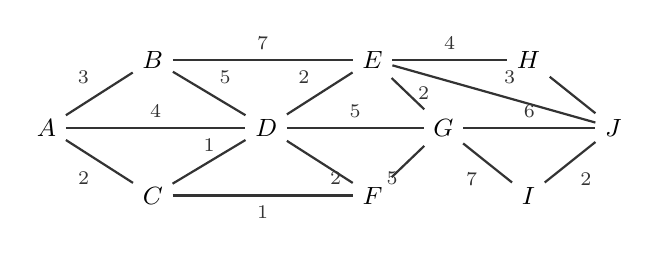
\begin{tikzpicture}[
  v/.style={font=\small},
  edge/.style={black!80,thick},
  every node/.style={font=\scriptsize},
  x=0.9cm,y=0.75cm
]
  \node[v] (a) at (0,0) {$A$};
  \node[v] (b) at (1.5,1.15) {$B$};
  \node[v] (c) at (1.5,-1.15) {$C$};
  \node[v] (d) at (3.1,0) {$D$};
  \node[v] (e) at (4.6,1.15) {$E$};
  \node[v] (f) at (4.6,-1.15) {$F$};
  \node[v] (g) at (5.6,0) {$G$};
  \node[v] (h) at (6.8,1.15) {$H$};
  \node[v] (i) at (6.8,-1.15) {$I$};
  \node[v] (j) at (8.0,0) {$J$};

  \draw[edge] (a)--node[above left]{3}(b);
  \draw[edge] (a)--node[above]{4}(d);
  \draw[edge] (a)--node[below left]{2}(c);
  \draw[edge] (b)--node[above]{7}(e);
  \draw[edge] (b)--node[above right]{5}(d);
  \draw[edge] (c)--node[above]{1}(d);
  \draw[edge] (c)--node[below]{1}(f);
  \draw[edge] (d)--node[above left]{2}(e);
  \draw[edge] (d)--node[above]{5}(g);
  \draw[edge] (d)--node[below right]{2}(f);
  \draw[edge] (e)--node[above]{4}(h);
  \draw[edge] (e)--node[right]{2}(g);
  \draw[edge] (e)--node[above right]{3}(j);
  \draw[edge] (f)--node[below left]{5}(g);
  \draw[edge] (g)--node[above]{6}(j);
  \draw[edge] (g)--node[below left]{7}(i);
  \draw[edge] (h)--(j);
  \draw[edge] (i)--node[below right]{2}(j);
\end{tikzpicture}\\[-0.2em]
{\small Hình 3. Ví dụ chi phí nhỏ nhất với giai đoạn không rõ ràng.}
\end{center}

\paragraph{Giải bài toán.}
Bài toán này không có cách chia giai đoạn rõ ràng; giữa các điểm không có thứ
tự trước sau cố định. Không thể quyết định thứ tự theo số bước ít nhất, vì đi
tắt từ $A$ đến $D$ tốn $4$, nhưng $A-C-D$ chỉ tốn $3$ và tốt hơn. Có vẻ như
trong đồ thị xuất hiện chu trình nên không thể dùng quy hoạch động. Thực ra
không phải vậy. Suy nghĩ kỹ, trong chiến lược tối ưu từ $A$ đến $J$, mỗi phần
của nó cũng là tối ưu (có thể chứng minh bằng phản chứng như trên). Nói cách
khác, bài này cũng có tính tối ưu, chỉ là giai đoạn không rõ ràng.

Với loại bài toán này, ta có thể đổi góc nhìn để phân tích và xây dựng thuật
toán. So với quy hoạch động tiến và lùi đã nói ở trên, cả hai đều lấy một
trạng thái nào đó làm điểm cuối, tìm các đường đi đến điểm ấy, rồi so sánh tốt
xấu để xác định giá trị tối ưu của trạng thái này. Nhưng trong bài này giai
đoạn không rõ; các đường giữa các trạng thái có thể lồng vào nhau, nên cách
đó không dùng được. Ta đổi góc nhìn: mỗi lần lấy một trạng thái làm điểm đầu,
duyệt các đường phát sinh từ nó. Khi mọi trạng thái đã biết đều được mở rộng
xong, ta mới so sánh mọi trạng thái mới, xác định trạng thái có giá trị nhỏ
nhất, còn các trạng thái khác giữ nguyên.

Trong Hình 3, trước hết xuất phát từ $A$, tìm được ba nút $B,D,C$ với chi phí
\[
  F(B)=3,\qquad F(D)=4,\qquad F(C)=2.
\]
Vì $F(B)$ và $F(D)$ đều lớn hơn $F(C)$, ta có thể khẳng định: không thể còn
đường nào xuất phát từ $B$ hoặc $D$ đến $C$ tốt hơn $A-C$. Như vậy giá trị tối
ưu của $F(C)$ được xác định. Nhưng liệu có đường từ $C$ đến $B$ hoặc $D$ tốt
hơn $A-B$ hay $A-D$ không thì vẫn chưa rõ. Tiếp tục, vì $A$ đã mở rộng xong,
ta chỉ bắt đầu từ $C$, thu được $A-C-D=3$ và $A-C-F=3$, nên giá trị $F(D)$
được cập nhật thành $3$. Lúc này có
\[
  F(B)=F(D)=F(F)=3,
\]
và giá trị tối ưu của cả ba điểm đều được xác định. Sau đó lần lượt lấy ba
điểm này làm điểm đầu để tiếp tục tìm kiếm. Cứ như vậy cho đến khi giá trị
tối ưu của điểm $J$ được xác định.

Quan sát kỹ, giai đoạn ẩn của bài này thực ra chính là sự phân chia theo độ
lớn của giá trị tối ưu của các nút. Quá trình trên là quy hoạch động tiến
theo thứ tự giá trị tối ưu tăng dần. Người ta thường xếp bài này vào phạm vi
lý thuyết đồ thị và gọi phương pháp trên là phương pháp gán nhãn.

\section{Ứng dụng của quy hoạch động}

Phần trên đã trình bày vài cách giải bằng quy hoạch động. Dưới đây ta dùng
các ví dụ để hiểu sâu hơn.

\subsubsection*{Ví dụ 4: sao chép bản thảo (BOOKS)}

\paragraph{Mô tả bài toán.}
Giả sử có $M$ cuốn sách, đánh số $1,2,\ldots,M$, và muốn sao chép mỗi cuốn
một bản. Số trang của $M$ cuốn có thể khác nhau, lần lượt là
$P_1,P_2,\ldots,P_M$. Nhiệm vụ là phân $M$ cuốn sách cho $K$ người chép
($K\le M$). Mỗi cuốn sách chỉ được phân cho một người chép, và các sách được
phân cho mỗi người chép phải liên tiếp theo thứ tự.

Nói cách khác, tồn tại một dãy tăng liên tiếp
\[
  0=b_0<b_1<b_2<\cdots<b_{k-1}<b_k=M,
\]
sao cho người chép số $i$ nhận các bản thảo từ cuốn $b_{i-1}+1$ đến cuốn
$b_i$. Công việc sao chép bắt đầu đồng thời, và tốc độ sao chép của mọi người
chép đều như nhau. Vì vậy thời gian cần để chép xong mọi bản thảo phụ thuộc
vào thời gian của người được phân nhiều việc nhất. Hãy tìm một phương án phân
tối ưu, sao cho giá trị lớn nhất trong tổng số trang được phân cho mỗi người
chép là nhỏ nhất có thể. Nếu có nhiều phương án tối ưu thì chỉ cần xuất một
phương án.

\paragraph{Giải bài toán.}
Trong bài này, $M$ cuốn sách được sắp theo thứ tự, và lựa chọn cho $K$ người
chép cũng có thứ tự, liên tiếp. Dù lấy chỉ số sách hay chỉ số người chép làm
tham số để chia giai đoạn, bài toán đều thỏa nguyên lý tối ưu của chiến lược
và tính không hậu hiệu. Do $K\le M$, chia theo chỉ số người chép sẽ tiện hơn.

Gọi $F(i,j)$ là giá trị nhỏ nhất của ``số trang lớn nhất'' khi $i$ người chép
đầu sao chép $j$ cuốn sách đầu. Khi đó có
\[
  F(i,j)=
  \min_{i-1\le v\le j-1}
  \max\{F(i-1,v),\;T(v+1,j)\},
\]
trong đó
\[
  1\le i\le K,\qquad i\le j\le M-K+i,
\]
và $T(v+1,j)$ biểu thị tổng số trang từ cuốn $v+1$ đến cuốn $j$. Điều kiện
đầu là $F(1,1)=P_1$.

Quan sát công thức truy hồi, ta thấy giai đoạn $F(i)$ chỉ phụ thuộc vào các
giá trị trạng thái của giai đoạn $F(i-1)$. Khi lập trình, có thể đặt phạm vi
của mảng $F$ là $(0\ldots1,1\ldots M)$ để giảm độ phức tạp bộ nhớ.

\subsubsection*{Ví dụ 5: quân domino (DOMINO)}

\paragraph{Mô tả bài toán.}
Có một loại quân domino phẳng, mặt trước được chia thành hai phần trên và
dưới. Mỗi phần hoặc trống, hoặc được đánh dấu từ $1$ đến $6$ chấm. Hiện có
một hàng quân domino đặt trên bàn. Trong ví dụ ở đề, tổng số chấm của hàng
trên là
\[
  6+1+1+1=9,
\]
còn tổng số chấm của hàng dưới là
\[
  1+5+3+2=11.
\]
Độ lệch giữa hai hàng là $2$, tức là giá trị tuyệt đối của hiệu hai tổng. Mỗi
quân domino đều có thể lật ngược trên dưới, tức phần trên trở thành phần dưới
và phần dưới trở thành phần trên.

Nhiệm vụ hiện tại là dùng số lần lật ít nhất để làm cho độ lệch giữa hàng
trên và hàng dưới nhỏ nhất. Với ví dụ trên, chỉ cần lật quân cuối cùng là có
thể làm độ lệch bằng $0$, nên đáp án của ví dụ là $1$.

\paragraph{Giải bài toán.}
Độ lệch có dấu giữa phần trên và phần dưới của ví dụ là
\[
\begin{aligned}
&6+1+1+1-(1+5+3+2)\\
&\quad=(6-1)+(1-5)+(1-3)+(1-2)=-2.
\end{aligned}
\]
Sau khi lật quân cuối cùng, hiệu trên dưới trở thành
\[
  (6-1)+(1-5)+(1-3)+(2-1)=0.
\]
Từ đó thấy rằng ảnh hưởng của một quân domino lên chiến lược lật chỉ nằm ở
hiệu giữa số trên và số dưới; bản thân hai số trên quân là thứ yếu. Như vậy,
trạng thái đặt của các quân trong ví dụ được rút từ $8$ số thành $4$ số:
\[
  5,\ -4,\ -2,\ -1.
\]
Khi lật, chỉ cần đổi số ở vị trí đó sang số đối của nó.

Trong bài này, vì thứ tự lật các quân không bị hạn chế, không thể chia giai
đoạn theo chỉ số quân domino. Làm thế nào? Với loại bài toán có giai đoạn ẩn,
ta có thể chia giai đoạn theo độ lớn của giá trị tối ưu của trạng thái. Do đó
ta lấy hiệu giữa hai phần trên dưới của dãy domino, ký hiệu $I$, làm trạng
thái; lấy số bước lật để đạt trạng thái ấy làm giá trị trạng thái, ký hiệu
$f(I)$. Khi đó có thể viết
\[
  f(I)=\min\{f(I+j)+1\},
\]
trong đó $-12\le j\le 12$, $j$ là số chẵn, và trạng thái hiện tại cần có một
quân domino với hiệu bằng $j/2$. Ở đây $I$ không tăng giảm vô hạn; phạm vi
của nó phụ thuộc vào tổng các hiệu số trong dãy domino ban đầu.

Khi quy hoạch động cụ thể, với ví dụ trên, ta bắt đầu từ $f(-2)=0$. Sau một
lần lật theo các trạng thái quân, có thể nhận được
\[
  f(-12)=1,\qquad f(6)=1,\qquad f(2)=1,\qquad f(0)=1.
\]
Vì đã xuất hiện $f(0)$ nên chương trình có thể kết thúc; nếu không, tiếp tục
mở rộng theo bốn trạng thái mới cho đến khi xuất hiện $f(0)$ hoặc không còn
sinh được trạng thái mới.

Lưu ý: ở mỗi trạng thái, ngoài số bước ít nhất, còn phải ghi lại cách đặt của
các quân khi đạt trạng thái ấy. Khi đến một trạng thái và phát hiện đã có một
chiến lược lật được ghi lại, ta lấy chiến lược có số bước nhỏ hơn.

\section{Tổng kết}

Quy hoạch động là một thuật toán hiệu quả. Nếu vận dụng thành công, nó sẽ làm
hiệu suất chương trình, cả thời gian lẫn không gian, có bước nhảy vọt về chất.
Vì vậy ta xem nó là một nội dung quan trọng trong tư tưởng thuật toán, cần nắm
vững và nghiên cứu sâu. Hy vọng bài viết này đem lại một chút gợi ý cho bạn
đọc.

\appendix
\section{Phụ lục}

\subsection*{Ví dụ 4}

\paragraph{Định dạng nhập.}
Dòng đầu của tệp gồm hai số nguyên $m$ và $k$:
\[
  1\le k\le m\le 500.
\]
Dòng thứ hai có $m$ số nguyên $P_1,P_2,\ldots,P_m$; các số nguyên này đều
dương và không vượt quá $1000000$. Hai số nguyên kề nhau được cách nhau bởi
một dấu cách.

\paragraph{Định dạng xuất.}
Tệp có $k$ dòng, mỗi dòng gồm hai số nguyên dương, cách nhau bởi dấu cách.
Hai số nguyên $a_i$ và $b_i$ ở dòng thứ $i$ biểu thị chỉ số bắt đầu và chỉ số
kết thúc của các bản thảo được phân cho người chép số $i$.

\paragraph{Chương trình.}
\begin{verbatim}
program books;
type tp=array[1..500] of integer;
     tc=array[1..500] of longint;
var c:array[1..500] of ^tp;
    {ghi duong di}
    f:array[0..1] of tc;
    {gia tri trang thai}
    t:tc;
    {tong so trang}
    cc:tp;
    {lien ket duong di}
    i,j,v,k,m,x,y,min,p1,p2:longint;
    f1,f2:text;

procedure init;
{phan nhap}
begin
  assign(f1,'books.dat');
  reset(f1);
  assign(f2,'books.out');
  rewrite(f2);
  readln(f1,m,k);
  if k=1 then
  begin
    writeln(f2,1,' ',m);
    close(f2);
    halt;
  end;
  {xu ly rieng khi k=1}
  for i:=1 to m do
  begin
    read(f1,j);
    if i=1 then t[1]:=j else
      t[i]:=t[i-1]+j;
    {cong don so trang}
  end;
  for i:=1 to k do
    new(c[i]);
end;

procedure main;
{thu tuc chinh}
begin
  p1:=1; f[1]:=t;
  {trang thai ban dau}
  for i:=2 to k-1 do
  {tinh theo cong thuc truy hoi}
  begin
    p2:=p1; p1:=1-p2;
    for j:=i to m-k+i do
    begin
      min:=maxlongint; y:=0;
      for v:=i-1 to j-1 do
      begin
        if f[p2,v]>t[j]-t[v] then x:=f[p2,v]
          else x:=t[j]-t[v];
        if x<min then begin min:=x; y:=v; end;
      end;
      f[p1,j]:=min;
      c[i]^[j]:=y;
    end;
  end;
  p2:=p1; p1:=1-p2;
  min:=maxlongint; y:=0;
  for i:=k-1 to m-1 do
  begin
    if f[p2,i]>t[m]-t[i] then x:=f[p2,i]
      else x:=t[m]-t[i];
    if x<min then begin min:=x; y:=i; end;
  end;
  {cuoi cung tim phuong an phan toi uu}
  for i:=k-1 downto 1 do
  begin
    cc[i]:=y;
    y:=c[i]^[y];
  end;
  {lien ket duong di}
  writeln(f2,1,' ',cc[1]);
  for j:=2 to k-1 do
    writeln(f2,cc[j-1]+1,' ',cc[j]);
  writeln(f2,cc[k-1]+1,' ',m);
  close(f2);
  {in ket qua}
end;

begin
  init;
  main;
end.
\end{verbatim}

\subsection*{Ví dụ 5}

\paragraph{Định dạng nhập.}
Dòng đầu của tệp là một số nguyên $n$ ($1\le n\le 1000$), biểu thị có $n$
quân domino xếp thành một hàng trên bàn. Tiếp theo có $n$ dòng, mỗi dòng gồm
hai số nguyên $a,b$ ($0\le a,b\le 6$), cách nhau bởi dấu cách. Ở dòng thứ
$i+1$, $a$ và $b$ lần lượt biểu thị số chấm ở phần trên và phần dưới của quân
domino thứ $i$; $0$ biểu thị phần trống.

\paragraph{Định dạng xuất.}
Chỉ có một số nguyên ở dòng đầu của tệp. Số nguyên này biểu thị số lần lật
domino ít nhất để làm cho độ lệch giữa tổng số chấm của hàng trên và hàng
dưới là nhỏ nhất.

\paragraph{Chương trình.}
\begin{verbatim}
program domino;
type tp=array[1..6] of integer;
var t:array[1..6000] of ^tp;
    {ghi trang thai dat domino}
    f:array[-6000..6000] of integer;
    {ghi so buoc it nhat de dat mot hieu so}
    l:array[1..6000] of integer;
    {hang doi mo rong}
    tt:tp;
    i,j,n,m,x,y,ft,re:integer;
    f1,f2:text;

procedure init;
{khoi tao chuong trinh}
begin
  assign(f1,'domino.dat');
  reset(f1);
  assign(f2,'domino.out');
  rewrite(f2);
  m:=0;
  ft:=0; re:=1; new(t[1]);
  fillchar(t[1]^,sizeof(t[1]^),0);
  fillchar(f,sizeof(f),0);
  fillchar(tt,sizeof(tt),0);
  readln(f1,n);
  for i:=1 to n do
  begin
    readln(f1,x,y);
    if x<>y then
    begin
      x:=x-y;
      inc(m,x);
      inc(tt[abs(x)]);
      if x>0 then inc(t[1]^[x]);
    end;
  end;
  if m=0 then
  begin
    writeln(f2,0);
    close(f2);
    halt;
  end;
  {xu ly truong hop so buoc bang khong}
  l[1]:=m;
  f[m]:=1;
end;

procedure main;
{thu tuc chinh}
begin
  repeat
    for ft:=ft+1 to re do
    {mo rong trang thai theo so buoc}
    begin
      x:=l[ft];
      for i:=1 to 6 do
      {sau truong hop hieu so khac nhau}
      begin
        if x<6 then
        if (t[ft]^[i]<tt[i])and(f[x+i*2]=0) then
        begin
          inc(re); l[re]:=x+i*2;
          f[l[re]]:=f[x]+1;
          if l[re]=0 then
          {tim duoc loi giai thi in}
          begin
            writeln(f2,f[l[re]]-1);
            close(f2);
            halt;
          end;
          new(t[re]);
          t[re]^:=t[ft]^;
          inc(t[re]^[i]);
        end;
        {hieu so tang}
        if x>-6 then
        if (t[ft]^[i]>0)and(f[x-i*2]=0) then
        begin
          inc(re); l[re]:=x-i*2;
          f[l[re]]:=f[x]+1;
          if l[re]=0 then
          {tim duoc loi giai thi in}
          begin
            writeln(f2,f[l[re]]-1);
            close(f2);
            halt;
          end;
          new(t[re]);
          t[re]^:=t[ft]^;
          dec(t[re]^[i]);
        end;
        {hieu so giam}
      end;
    end;
  until ft=re;
  for i:=1 to 6 do
  if (f[i]>0)or(f[-i]>0) then
  begin
    if (f[-i]>0)and((f[i]=0)or(f[-i]<f[i])) then x:=f[-i]
      else x:=f[i];
    writeln(f2,x-1);
    i:=6;
  end;
  close(f2);
  {gia tri tuyet doi cua hieu hai tong khong bang khong}
end;

begin
  init;
  main;
end.
\end{verbatim}

\end{document}
